\beginsong{Heute hier, morgen dort}[
    wuw={Hannes Wader}, 
    jahr={1972}, 
    bo={180}, 
    pfii={99}, 
    pfiii={29}, 
    kssiv={82}, 
    siru={99},
    tonspur={294}, 
]

\beginverse
\endverse
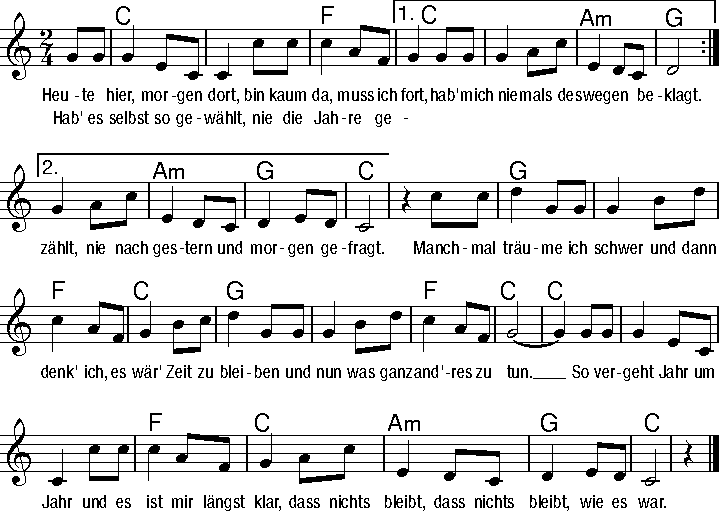
\includegraphics[draft=false, width=1\textwidth]{Noten/Lied050.pdf}	

\beginverse
Dass man \[C]mich kaum vermisst, schon nach \[F]Tagen ver\[C]gisst,
wenn ich längst wieder \[Am]anderswo \[G]bin,
stört und \[C]kümmert mich nicht, vielleicht \[F]bleibt mein Ge\[C]sicht
doch dem \[Am]ein' oder \[G]and'ren im \[C]Sinn.
\endverse

\beginchorus
Manchmal \[G]träume ich schwer und dann \[F]denk' ich, es \[C]wär'
Zeit zu \[G]bleiben und nun was ganz \[F]and'res zu \[C]tun.
So vergeht Jahr um Jahr und es \[F]ist mir längst \[C]klar,
dass nichts \[Am]bleibt, dass nichts \[G]bleibt, wie es \[C]war.
\endchorus

\beginverse
Fragt mich ^einer, warum ich so ^bin, bleib ich ^stumm,
denn die Antwort da^rauf fällt mir ^schwer.
Denn was ^neu ist, wird alt, und was ^gestern noch ^galt,
stimmt schon ^heut' oder ^morgen nicht ^mehr.
\endverse

\printchorus

\endsong

\beginscripture{}
Die Melodie zu ''Heute hier, morgen dort'' entstammt dem Song ''Indian Summer'' des Musikers Gary Bolstad um 1960. Hannes Wader schrieb zur Melodie, die er in einem Berliner Folkclub aufschnappte, den heute bekannten Text. Gary Bolstad übersetzte 1997 den deutschen Text von Hannes Wader wiederum ins Englische. 
Das Lied knüpft thematisch an das Gefühl in der Wandervogelbewegung an.
\endscripture
